\chapter{Hardware}

\section{Schéma structurel}

Ci-dessous le schéma structurel de la carte électronique du télescope. Un accès d'alimentation $+12V$ pour un ventilateur a été ajouté, celui-ci étant normalement présent sous le miroir primaire et servant à le garder à température constante. Il avait été oublié jusqu'à présent.

\begin{figure}[H]
    \centering
    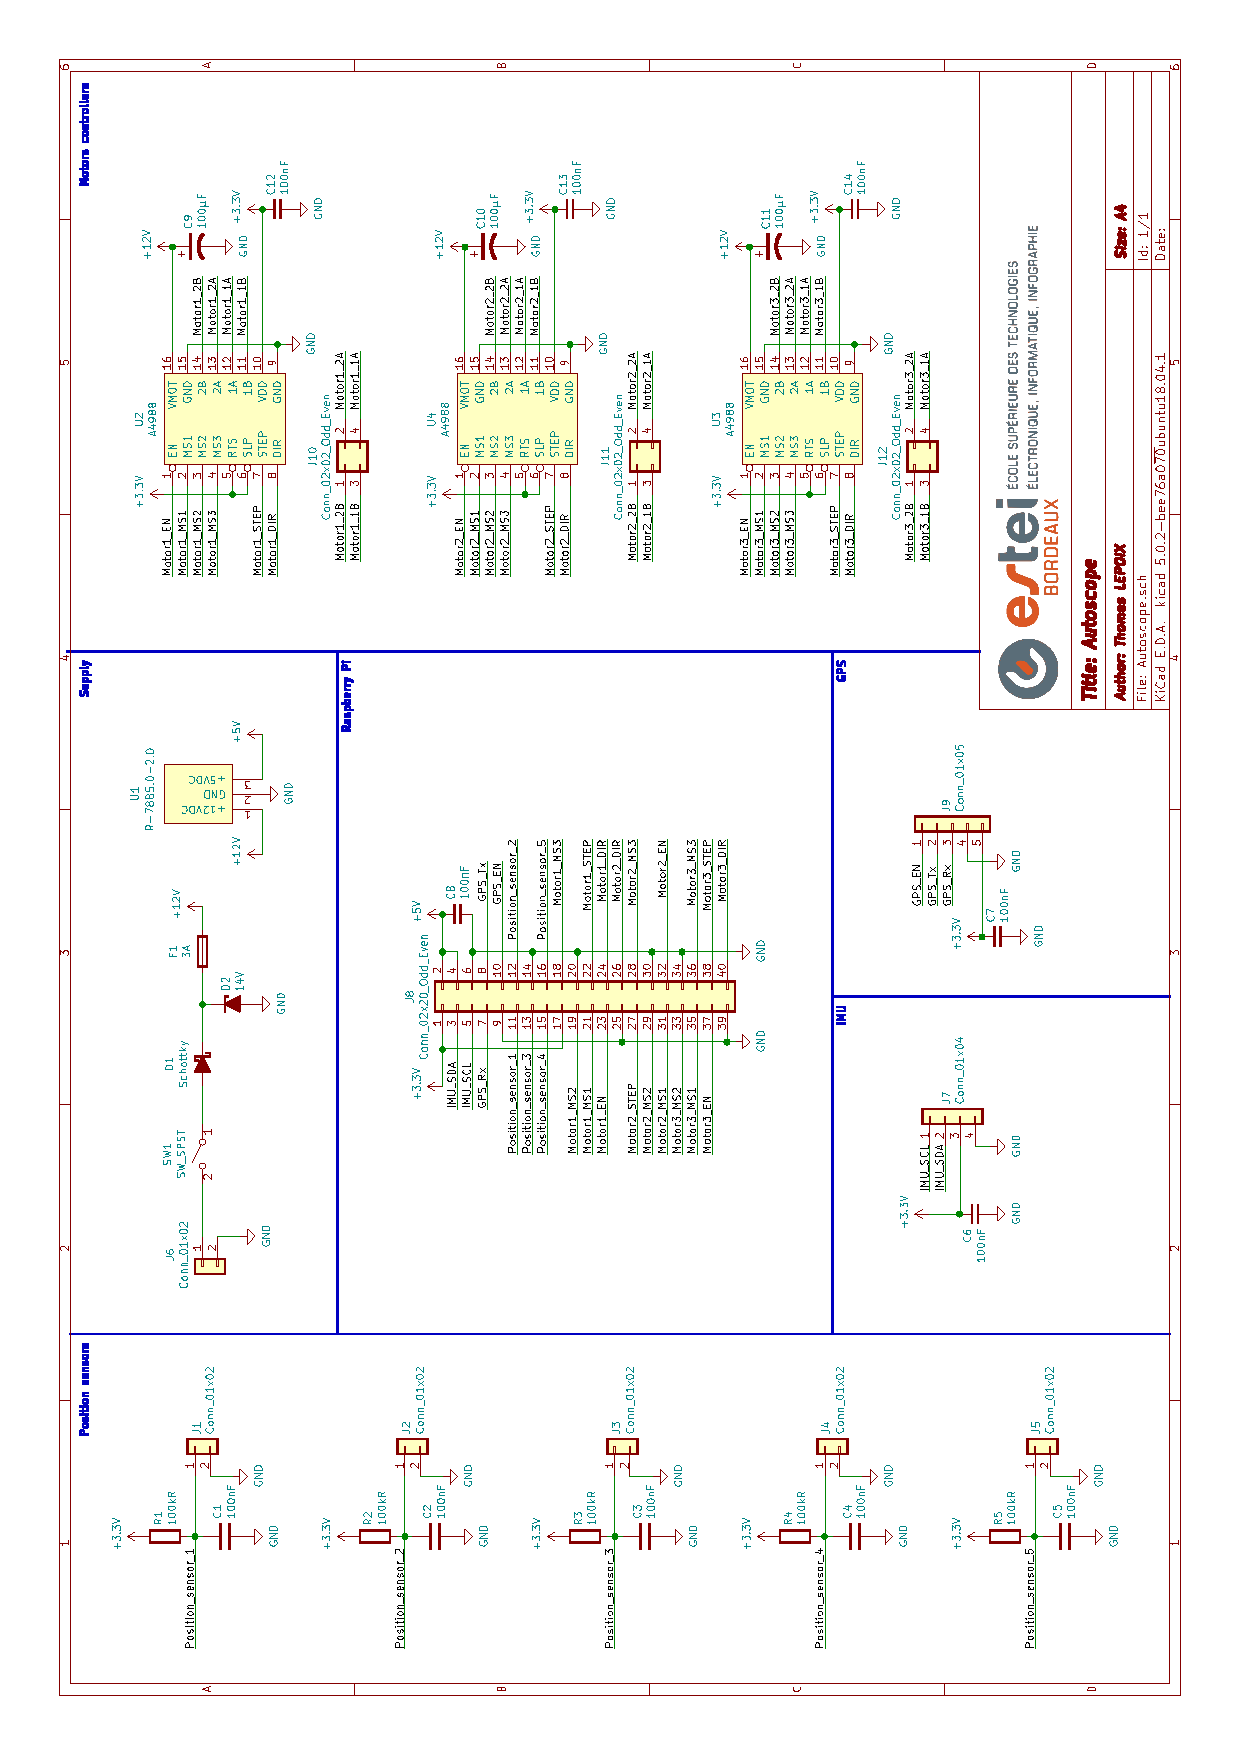
\includegraphics[width=1\linewidth]{\figures/kicad_sch.pdf}
    \decoRule
    \caption[
    Schéma structurel de la carte du télescope]{
    Schéma structurel de la carte du télescope}
    \label{fig:Schéma structurel de la carte du télescope}
    \end{figure}

\newpage
\section{Bon de commande}

Figurent sur le bon de commande tous les éléments faisant partie du télescope, on observe ainsi le prix de chaque partie~:
\begin{itemize}[label=$\bullet$]
	\item Éléments optiques~: $454$€
	\item Motorisation~: $64,7$€
	\item Système électronique~: $197,49$€ dont~:
	\begin{itemize}
		\item Raspberry-Pi et carte mémoire~: $39,09$€
		\item Carte électronique Autoscope~: $158,40$€
		\end{itemize}
	\end{itemize}

\vspace{1cm}

Le vert représente les composants déjà reçus, le jaune ceux commandés et le orange ceux qui seront considérés plus tard.

\begin{figure}[H]
    \centering
    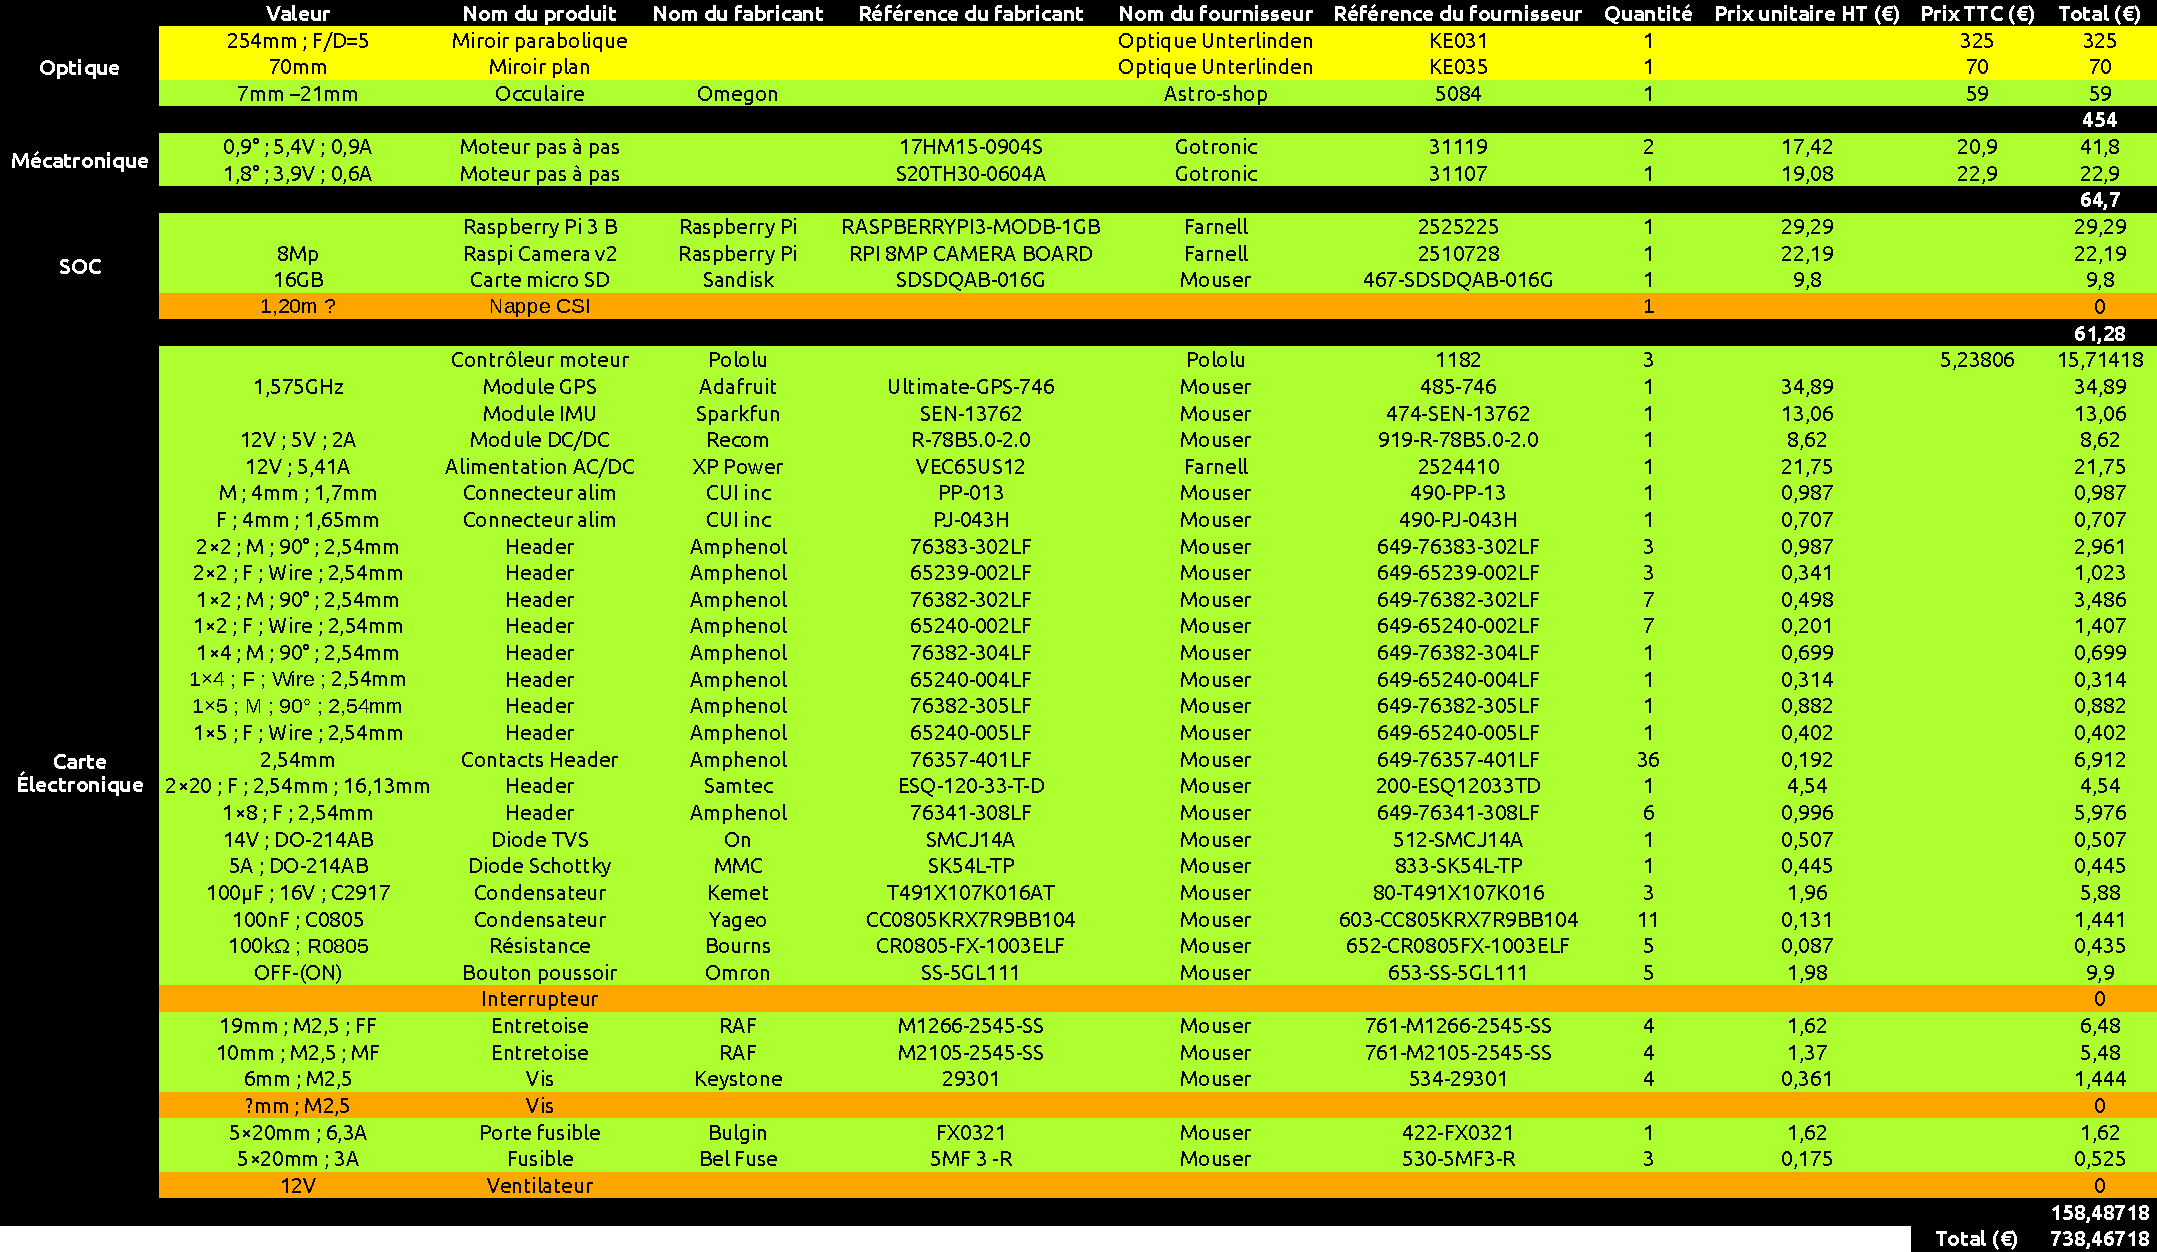
\includegraphics[width=1\linewidth]{\figures/tab_bom.pdf}
    \decoRule
    \caption[
    Bon de commande du matériel du télescope]{
    Bon de commande du matériel du télescope}
    \label{fig:Bon de commande du matériel du télescope}
    \end{figure}

\section{Fichiers de fabrication}

\begin{figure}[H]
    \centering
    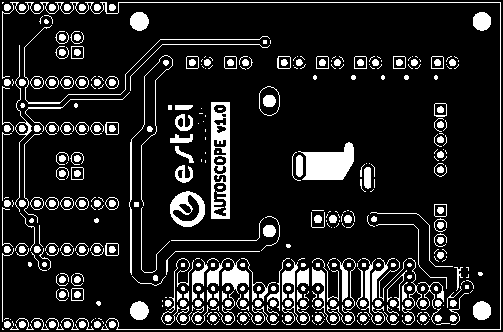
\includegraphics[width=0.49\linewidth]{\figures/kicad_f2.pdf}
    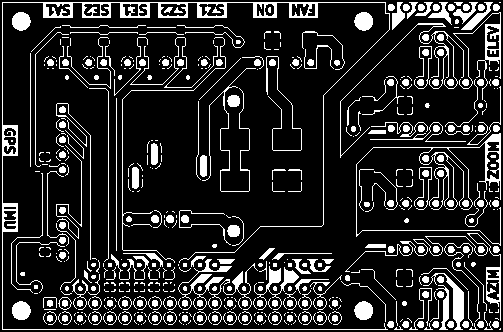
\includegraphics[width=0.49\linewidth]{\figures/kicad_b2.pdf}
    \decoRule
    \caption[
    Faces supérieure et inférieure du typon de la carte\\(respectivement vues de dessus et de dessous)]{
    Faces supérieure et inférieure du typon de la carte\\(respectivement vues de dessus et de dessous)}
    \label{fig:Faces supérieure et inférieure du typon de la carte (respectivement vues de dessus et de dessous)}
    \end{figure}

\begin{figure}[H]
    \centering
    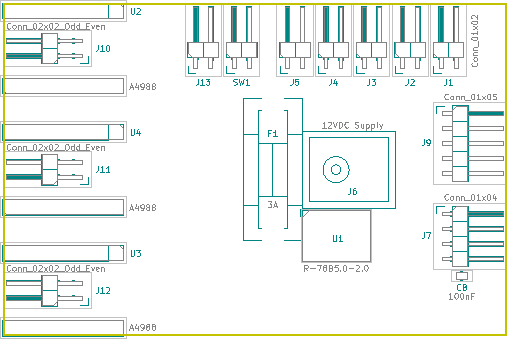
\includegraphics[width=0.49\linewidth]{\figures/kicad_cf.pdf}
    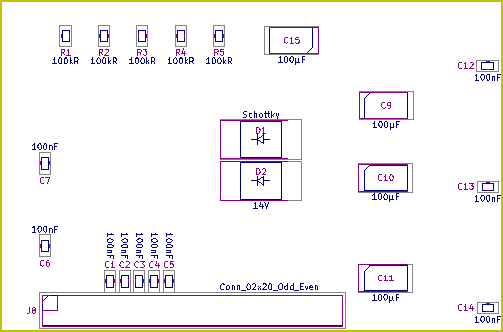
\includegraphics[width=0.49\linewidth]{\figures/kicad_cb.pdf}
    \decoRule
    \caption[
    Faces supérieure et inférieure de l'implantation des composants\\(respectivement vues de dessus et de dessous)]{
    Faces supérieure et inférieure de l'implantation des composants\\(respectivement vues de dessus et de dessous)}
    \label{fig:Faces supérieure et inférieure de l'implantation des composants (respectivement vues de dessus et de dessous)}
    \end{figure}

\section{Modélisation 3D}

\begin{figure}[H]
    \centering
    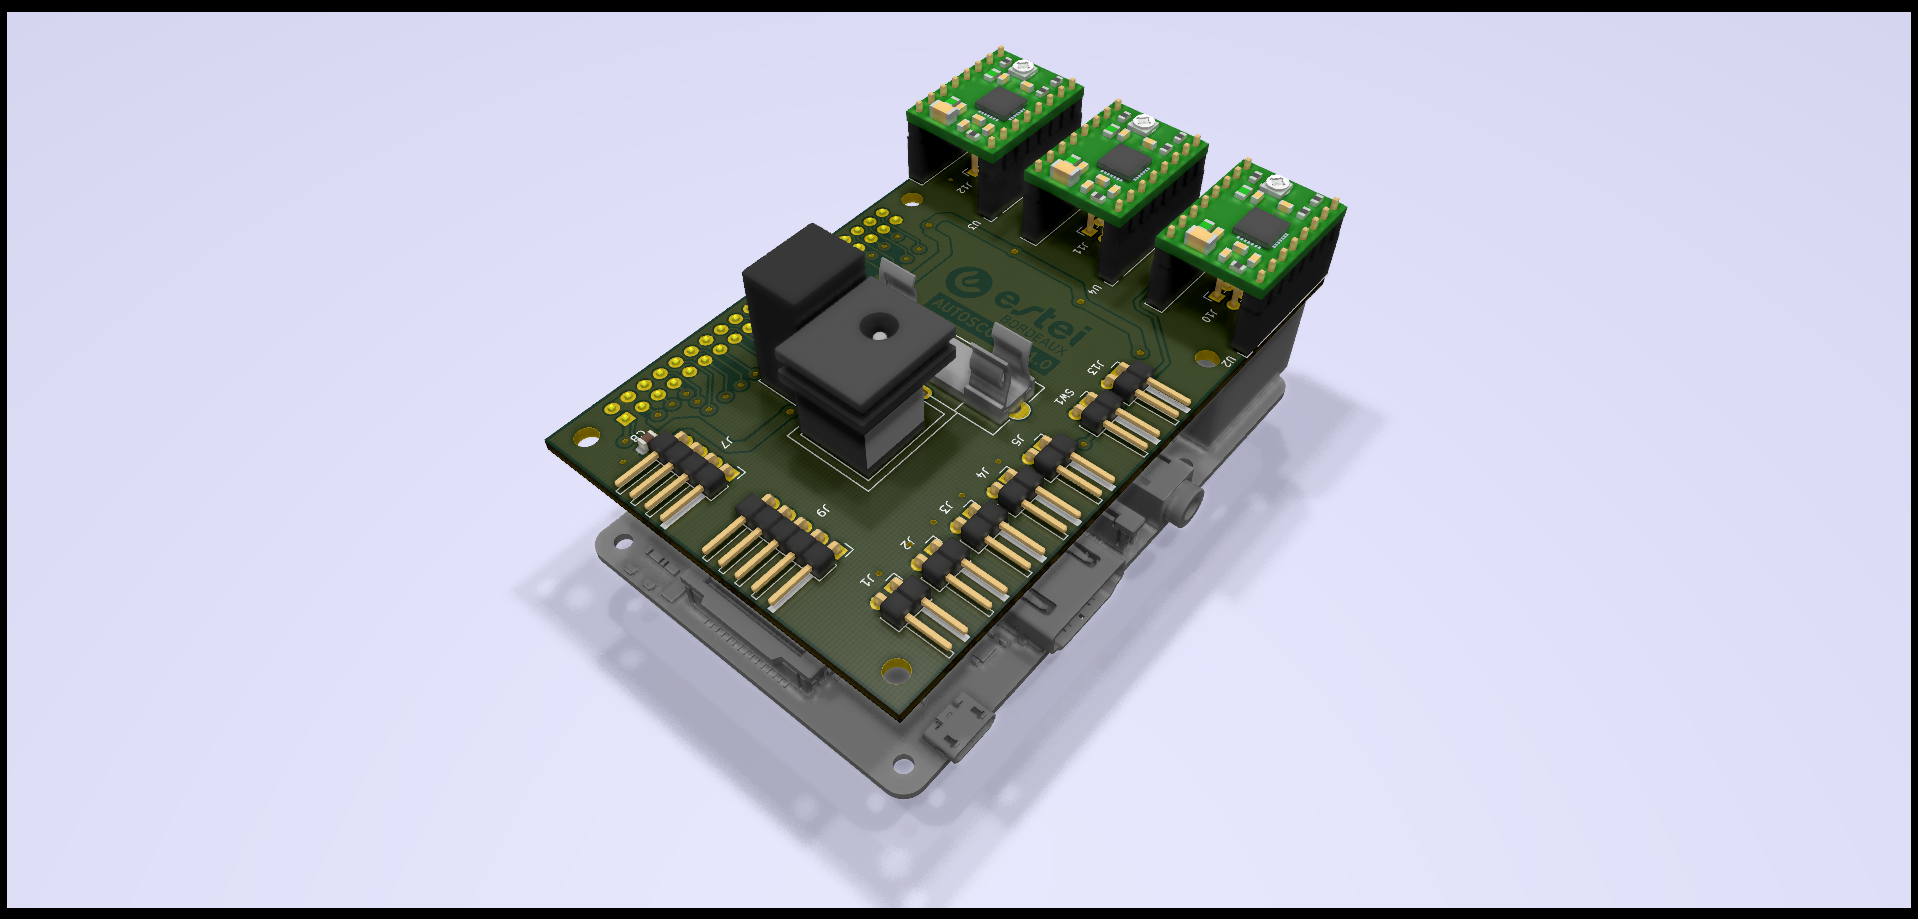
\includegraphics[width=1\linewidth]{\figures/kicad_3d_3.png}
    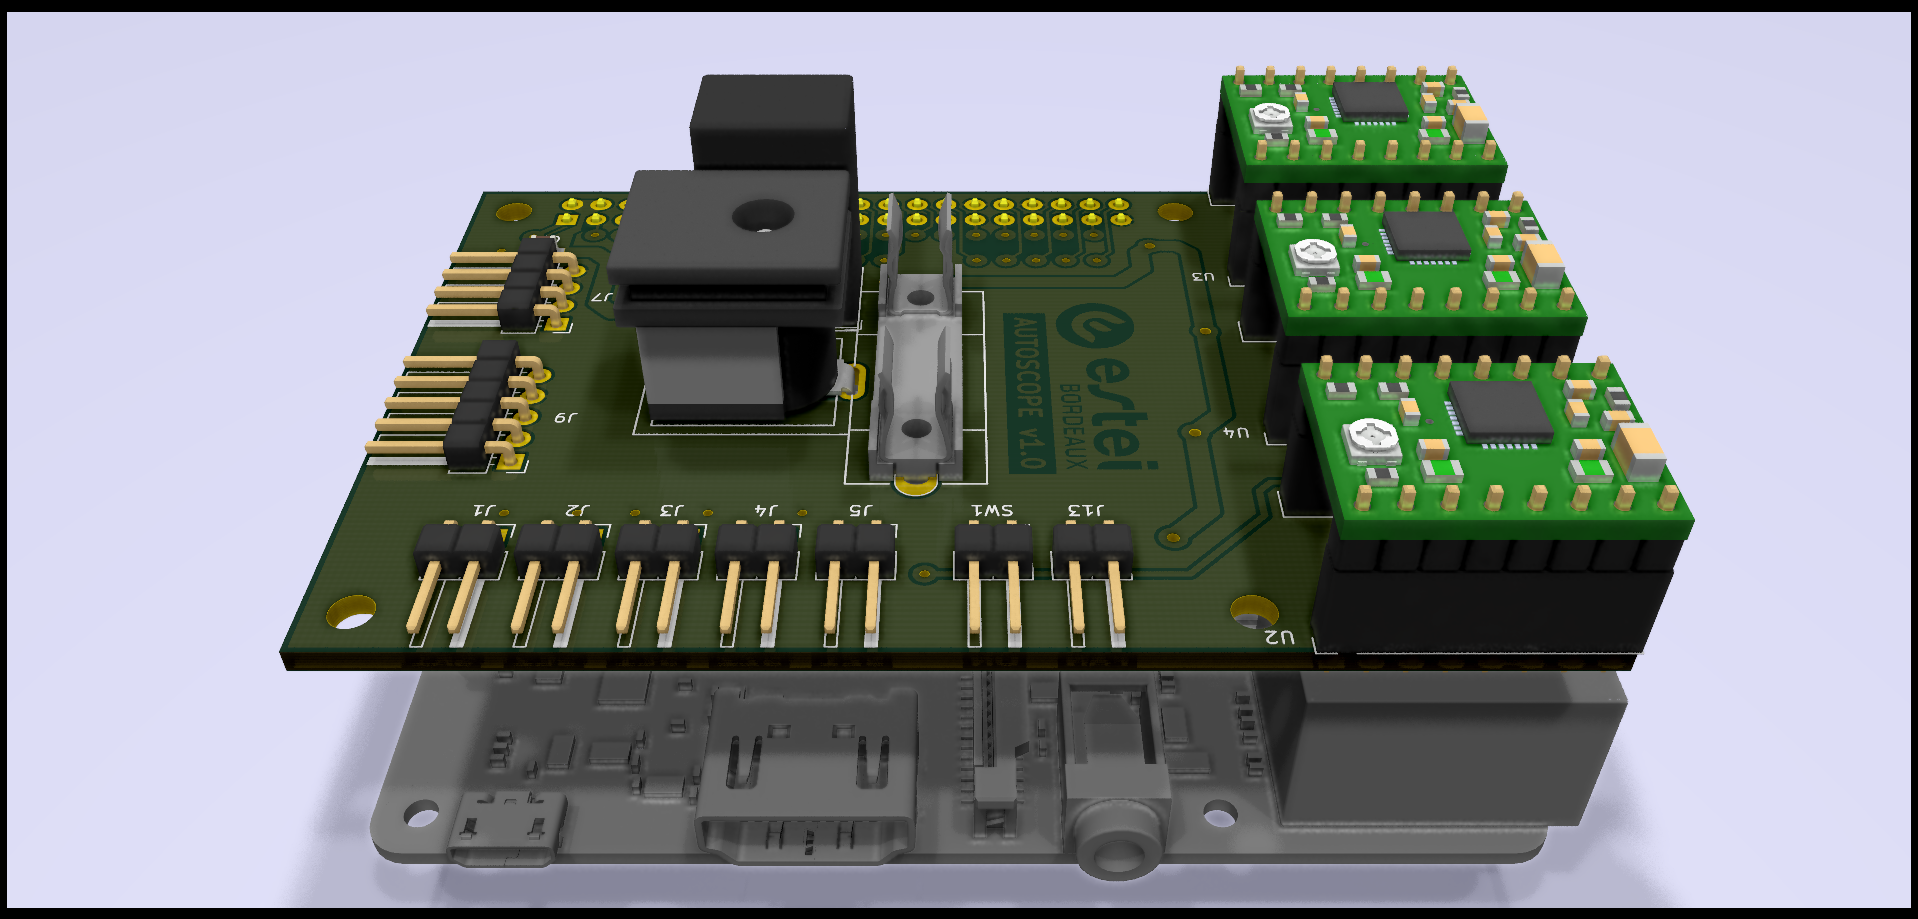
\includegraphics[width=0.495\linewidth]{\figures/kicad_3d_2.png}
    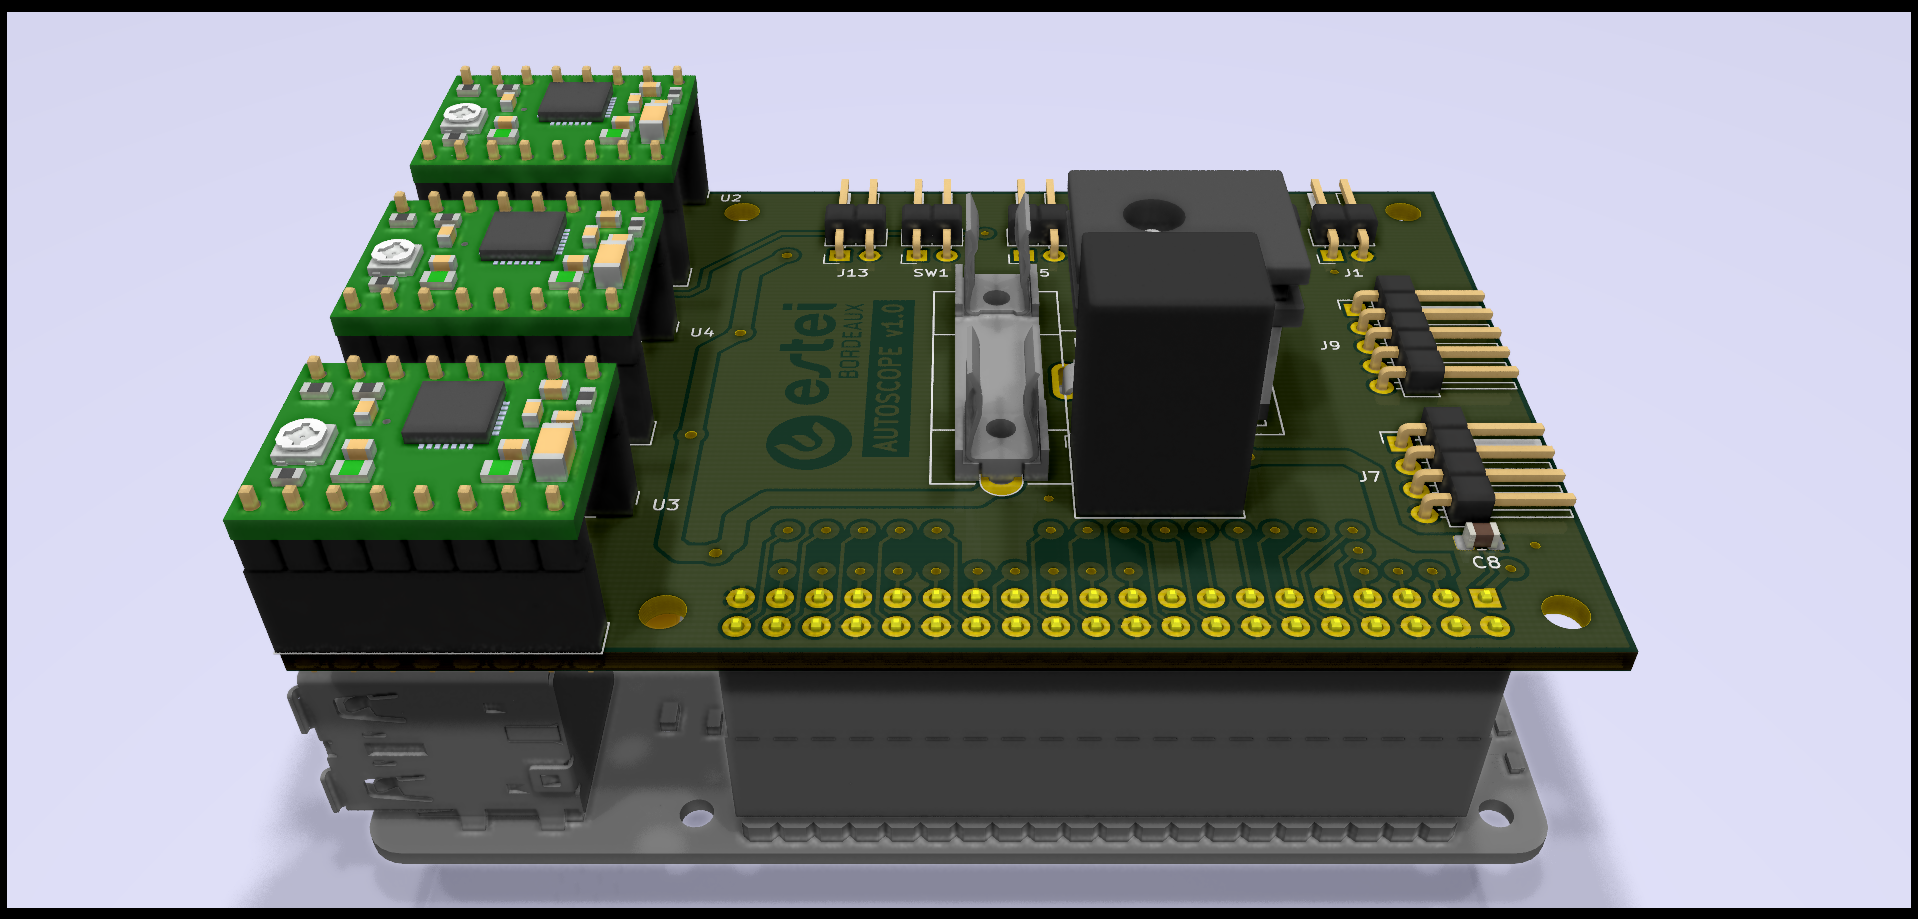
\includegraphics[width=0.495\linewidth]{\figures/kicad_3d_1.png}
    \decoRule
    \caption[
    Modélisation 3D de la carte pluggée sur la Raspberry-Pi]{
    Modélisation 3D de la carte pluggée sur la Raspberry-Pi}
    \label{fig:Modélisation 3D de la carte pluggée sur la Raspberry-Pi}
    \end{figure}

\vspace{1cm}

Au delà de l'aspect esthétique, la modélisation 3D permet d'avoir un aperçu du produit fini et de valider ou non le respect de certaines contraintes de design. Ou encore de repérer des vices que l'on ne voit pas forcément lors de la réalisation du typon, voire du schéma.

%\vspace{1cm}
\subsection{Allure générale de la carte}

Ainsi l'on observe d'abord l'allure générale de la carte~:

\begin{figure}[H]
    \centering
    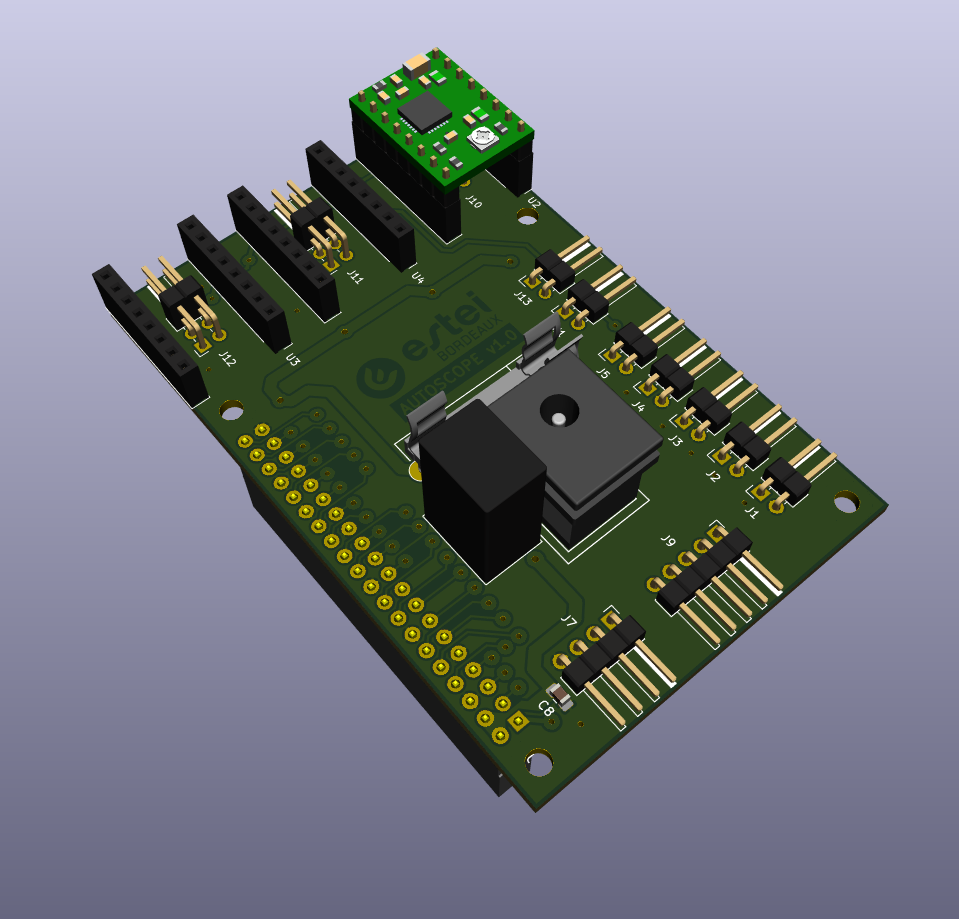
\includegraphics[width=0.49\linewidth]{\figures/kicad_3d_11_2.png}
    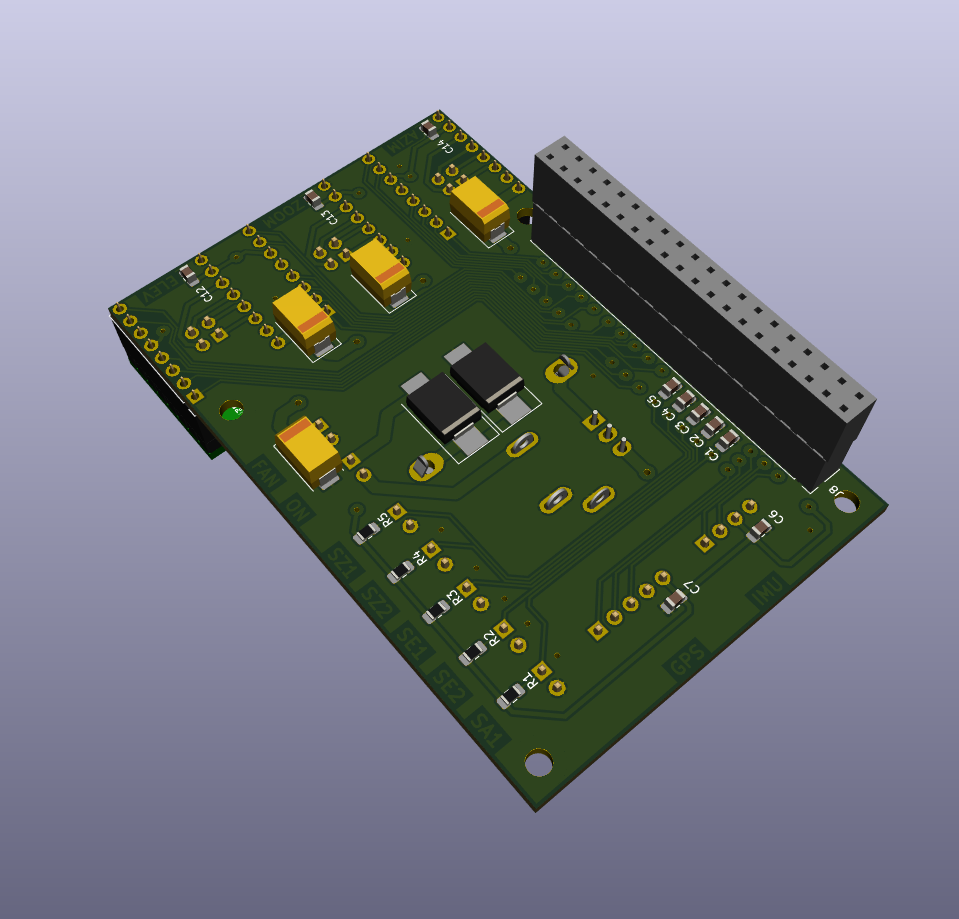
\includegraphics[width=0.49\linewidth]{\figures/kicad_3d_12_2.png}
    \decoRule
    \caption[
    Modélisation 3D de la carte avec et sans modules de contrôle moteur]{
    Modélisation 3D de la carte avec et sans modules de contrôle moteur}
    \label{fig:Modélisation 3D de la carte avec et sans modules de contrôle moteur}
    \end{figure}

%\vspace{1cm}
\subsection{Connecteurs des moteurs}

Ensuite l'on peut s'assurer de la pertinence de disposer les connecteurs des moteurs sous leurs contrôleurs~:

\begin{figure}[H]
    \centering
    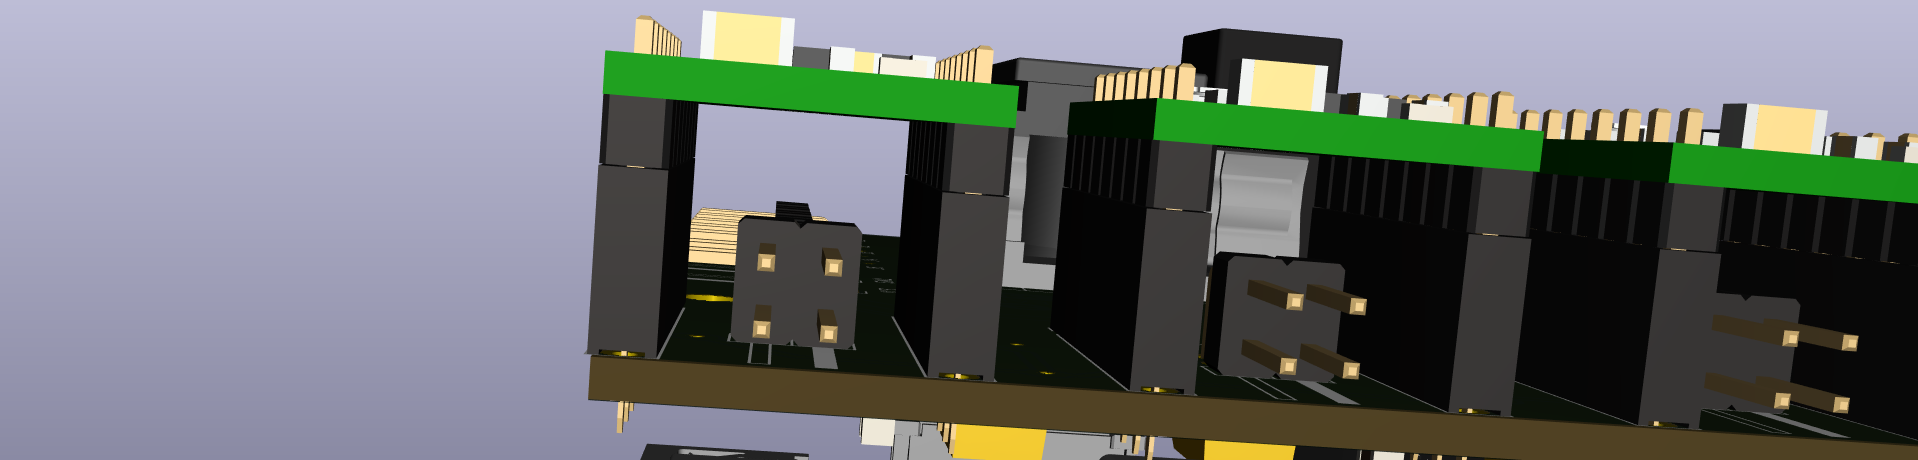
\includegraphics[width=1\linewidth]{\figures/kicad_3d_5_2.png}
    \decoRule
    \caption[
    Modélisation 3D de la carte~: zoom sur les connecteurs moteurs]{
    Modélisation 3D de la carte~: zoom sur les connecteurs moteurs}
    \label{fig:Modélisation 3D de la carte : zoom sur les connecteurs moteurs}
    \end{figure}

%\vspace{1cm}
\subsection{Emboîtement des cartes}

Puis on peut vérifier le correct emboîtement des cartes pour un espace les séparant de $19mm$, la longueur des entretoises utilisées. En particulier au niveau des condensateurs les plus volumineux~:

\begin{figure}[H]
    \centering
    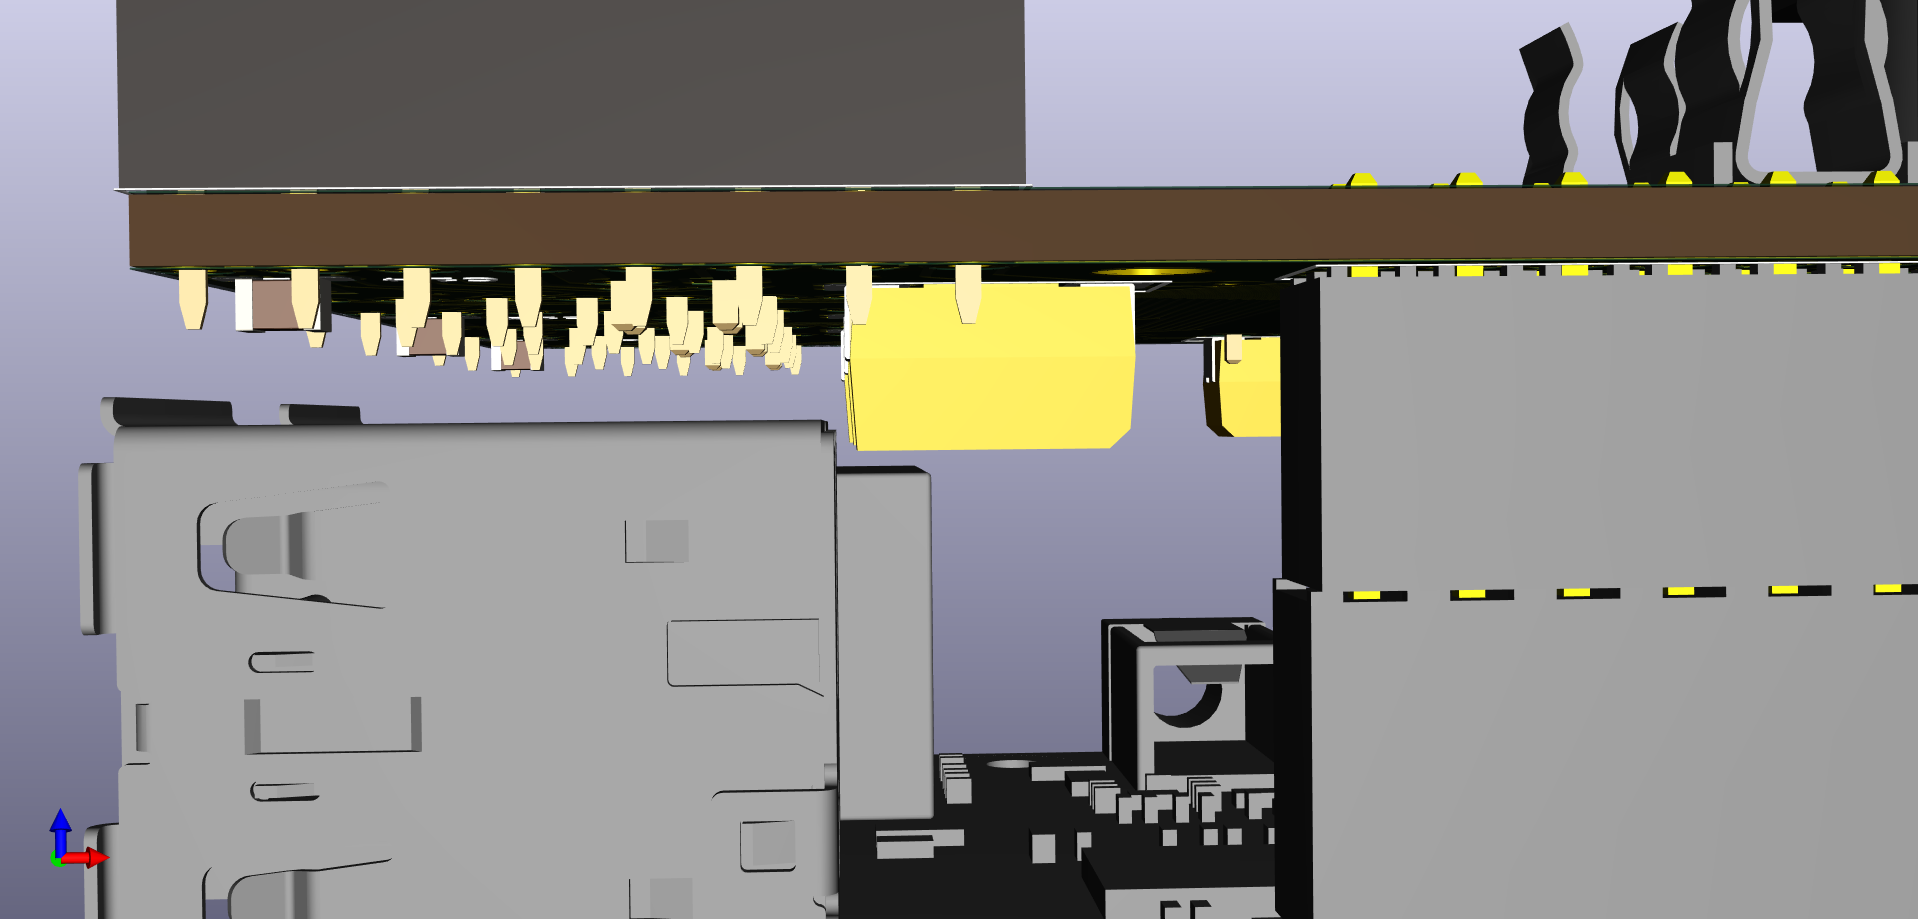
\includegraphics[width=0.49\linewidth]{\figures/kicad_3d_7_.png}
    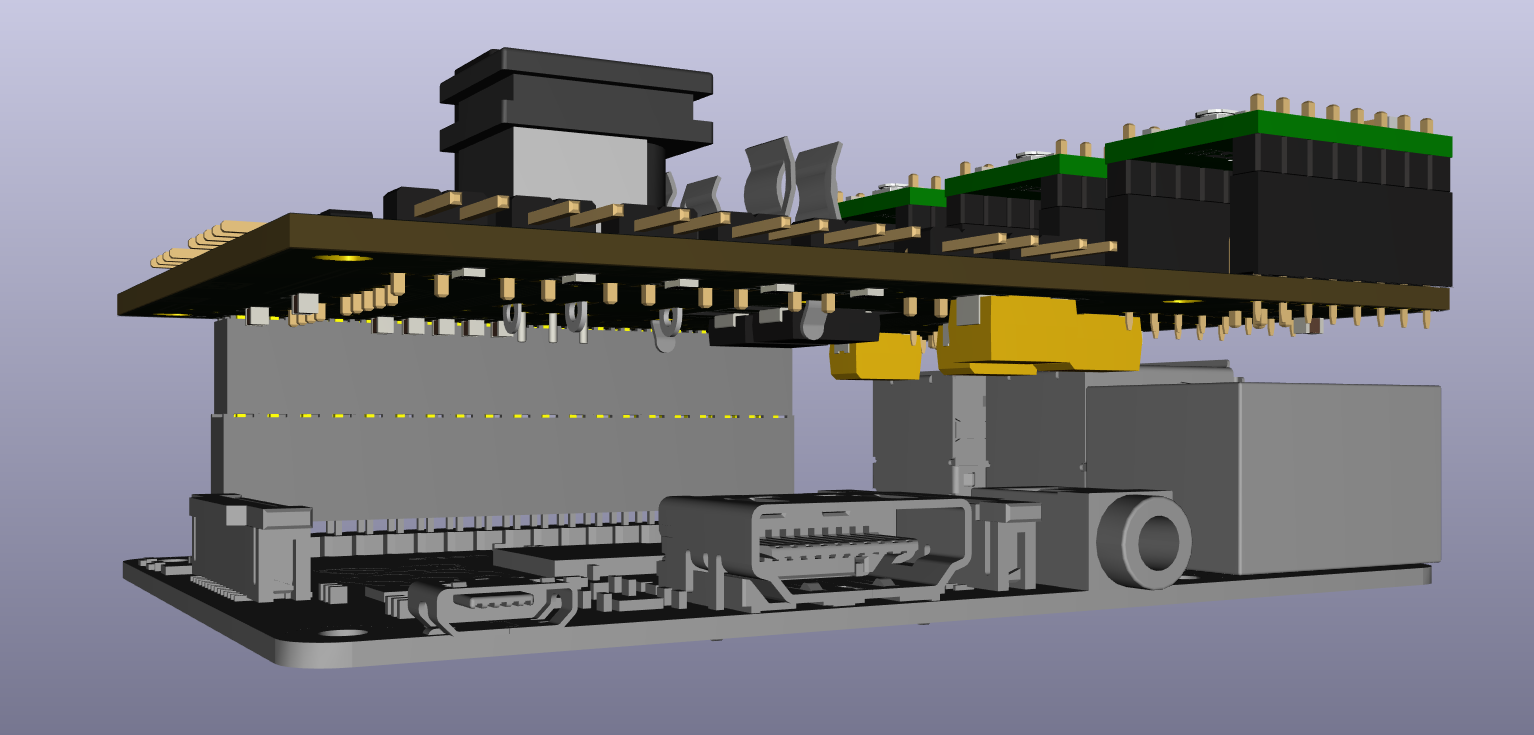
\includegraphics[width=0.49\linewidth]{\figures/kicad_3d_13_2.png}
    \decoRule
    \caption[
    Modélisation 3D de la carte~: zoom sur l'emboîtement des cartes]{
    Modélisation 3D de la carte~: zoom sur l'emboîtement des cartes}
    \label{fig:Modélisation 3D de la carte : zoom sur l'emboîtement des cartes}
    \end{figure}

%\vspace{1cm}
\subsection{Repères des connecteurs}

Enfin, question de commodité, des repères ont étés ajoutés pour indiquer le rôle de chaque connecteur. Ceux-ci se trouvent au niveau du connecteur associé, sur la face opposée du PCB, c'est-à-dire, sur la face coté Raspberry-Pi.

Placées sur le télescope, la Raspberry-Pi étant vouée à être sur le dessus, les repères sont sensés êtres visibles par l'utilisateur.

\begin{figure}[H]
    \centering
    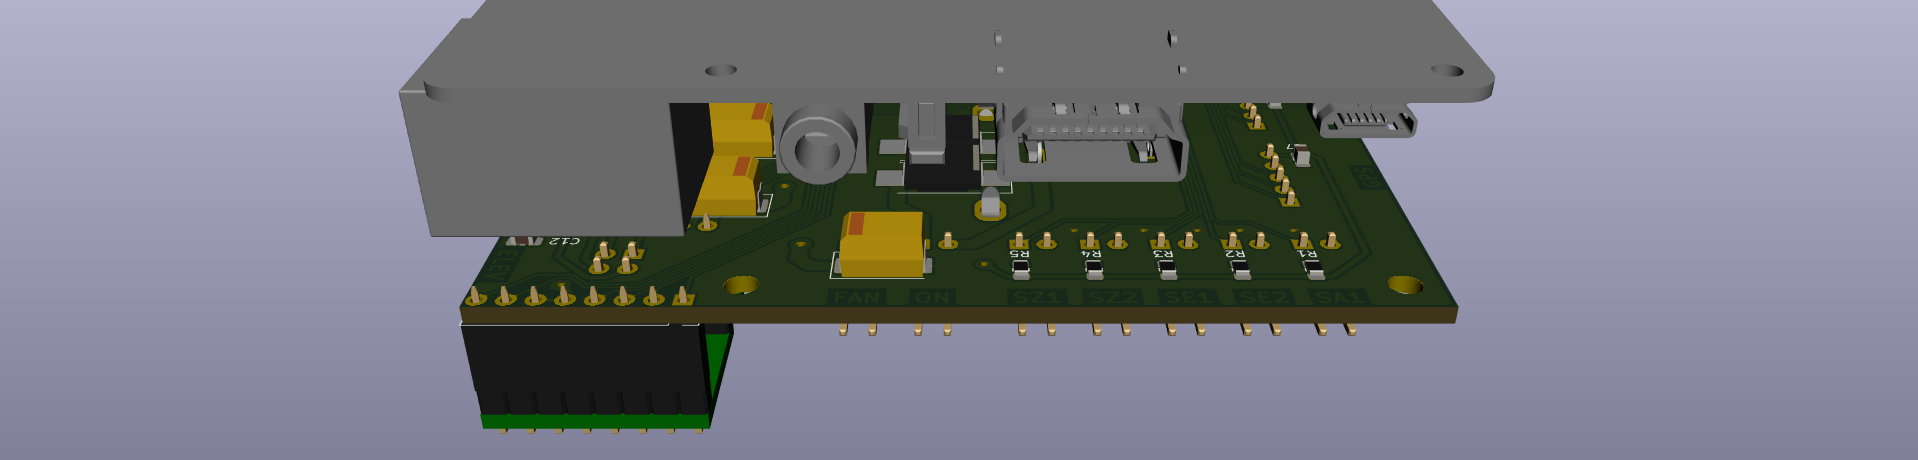
\includegraphics[width=1\linewidth]{\figures/kicad_3d_9_2.png}
    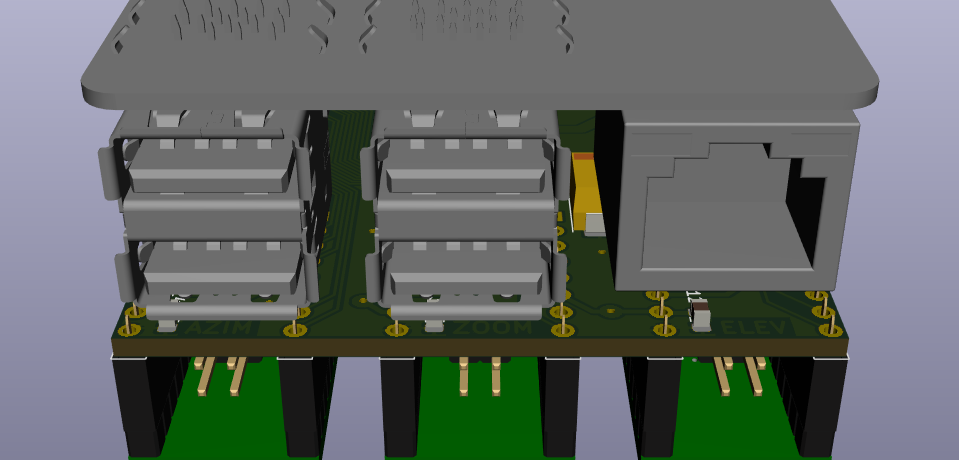
\includegraphics[width=0.495\linewidth]{\figures/kicad_3d_8_2.png}
    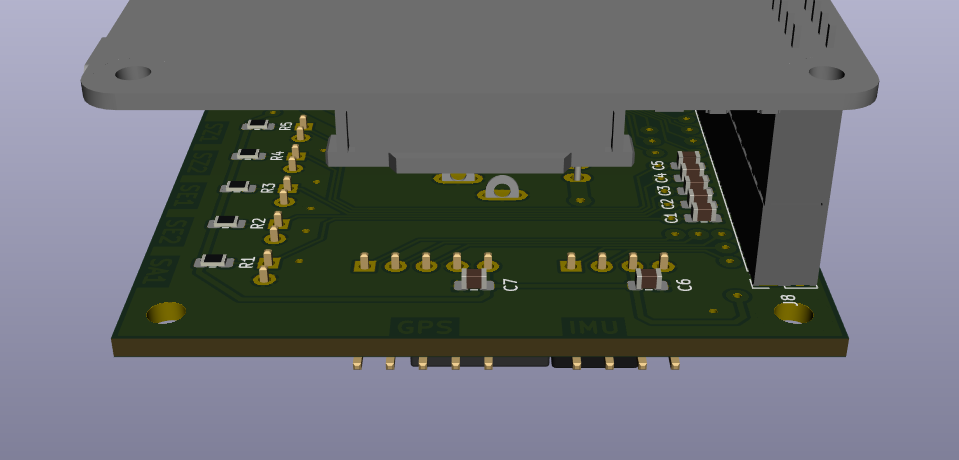
\includegraphics[width=0.495\linewidth]{\figures/kicad_3d_10_2.png}
    \decoRule
    \caption[
    Modélisation 3D de la carte~: zoom sur les repères des connecteurs]{
    Modélisation 3D de la carte~: zoom sur les repères des connecteurs}
    \label{fig:Modélisation 3D de la carte : zoom sur les repères des connecteurs}
    \end{figure}

\vspace{1cm}

\begin{itemize}[label=$\bullet$]
	\item AZIM~: Connecteur du moteur d'azimut.
	\item ZOOM~: Connecteur du moteur de zoom.
	\item ELEV~: Connecteur du moteur d'élévation.
	\item FAN~: Connecteur d'alimentation du ventilateur de refroidissement du miroir primaire.
	\item ON~: Connecteur d'un interrupteur On/Off d'alimentation du télescope.
	\item SZ1~: Connecteur du premier interrupteur de butée du moteur de zoom.
	\item SZ2~: Connecteur du second interrupteur de butée du moteur de zoom.
	\item SE1~: Connecteur du premier interrupteur de butée du moteur d'élévation.
	\item SE2~: Connecteur du second interrupteur de butée du moteur d'élévation.
	\item SA1~: Connecteur de l'unique interrupteur du moteur d'azimut.
	\item GPS~: Connecteur du module GPS.
	\item IMU~: Connecteur du module IMU (centrale inertielle).
	\end{itemize}

\subsection{Intégration du modèle 3D au télescope}

Il est possible d'exporter le modèle 3D des deux cartes emboîtées et ainsi de l'utiliser comme élément lors de la modélisation du télescope. Ci-dessous un aperçu des cartes grossièrement placées sur le modèle du télescope~:

\begin{figure}[H]
    \centering
    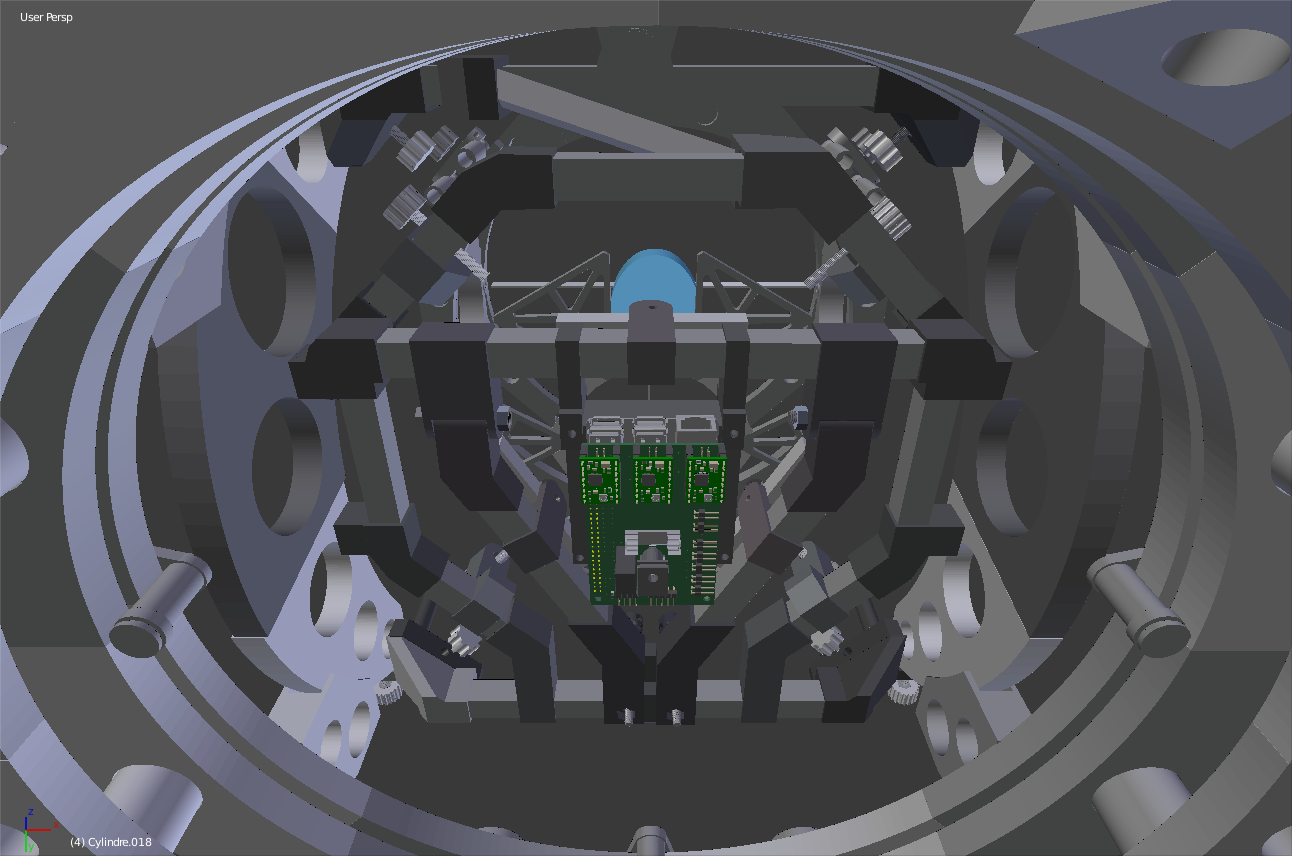
\includegraphics[width=0.495\linewidth]{\figures/blender_1.png}
    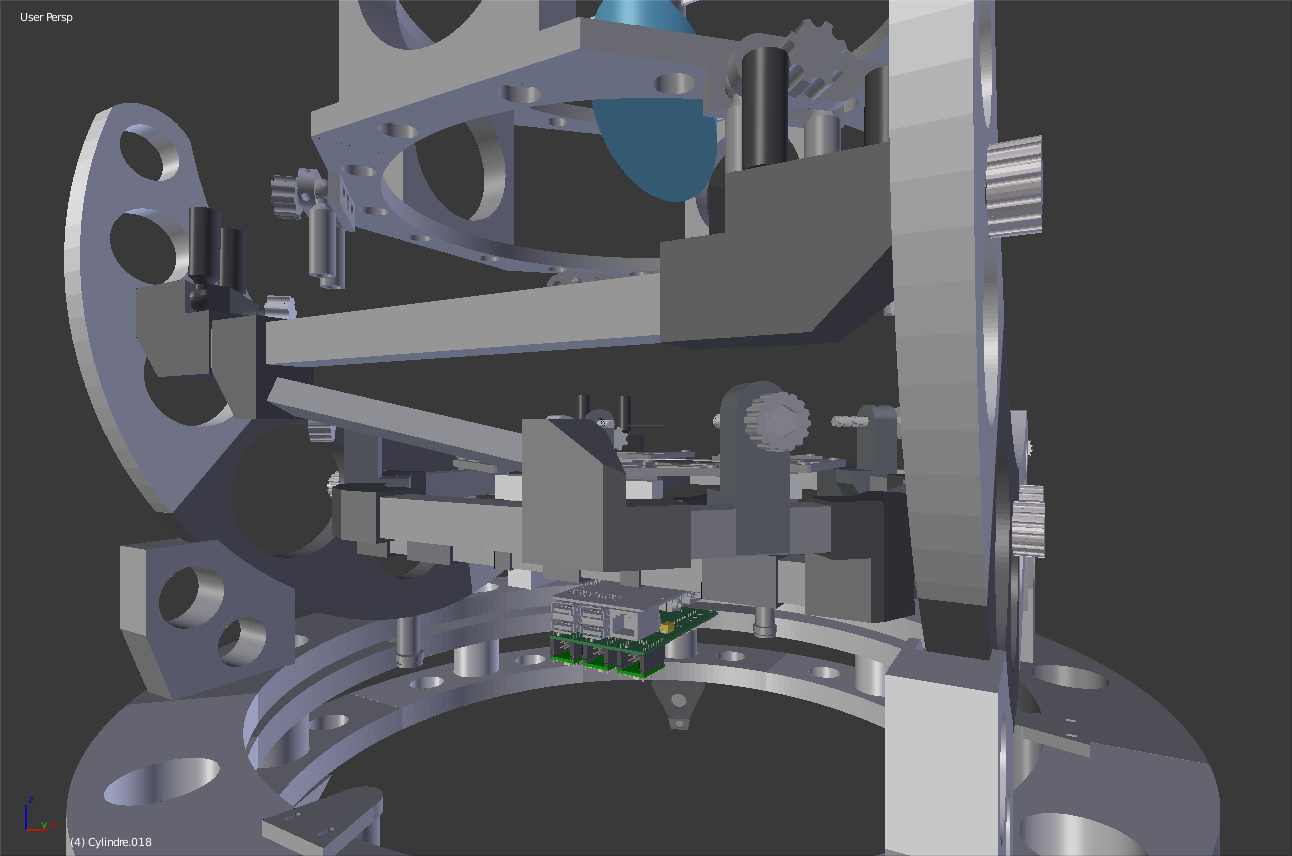
\includegraphics[width=0.495\linewidth]{\figures/blender_2.png}
    \decoRule
    \caption[
    Modélisation 3D du télescope grossièrement équipé de ses cartes électroniques]{
    Modélisation 3D du télescope grossièrement équipé de ses cartes électroniques}
    \label{fig:Modélisation 3D du télescope grossièrement équipé de ses cartes électroniques}
    \end{figure}
